\documentclass[12pt]{article}
\usepackage[english]{babel}
\usepackage{amssymb}
\usepackage{amsmath}
\usepackage{mathrsfs}
\usepackage[pdftex]{graphicx}
\usepackage[left=20mm, top=10mm, right=20mm, bottom=15mm]{geometry}
\usepackage{graphics}
\usepackage{gensymb}



\title{Laboratory work 1.4.2\\Determination of the acceleration of free fall using a revolving pendulum}
\author{\textbf{Author: Vorobev Igor}}

\begin{document}
\maketitle
\textbf{The purpose of the work}: using a revolving pendulum, measure the magnitude of the acceleration of free fall.\\

\textbf{Equipment}: a revolving pendulum with two suspended prisms and two weights (lentils); an electronic counter of time and number of oscillations; a stand with a point for determining the position of the center of mass of the pendulum; a wall-mounted console for hanging the pendulum; metal rulers, a caliper 1 m long.\\

\textbf{\large Theory}


A physical pendulum is a solid body capable of oscillating in a vertical plane. 

For small fluctuations , the oscillation period of the physical pendulum: $$T = 2\pi\sqrt{\frac{I}{mgl}}\quad (1)$$ where $I$ - moment of inertia, $m$ - weight, $l$ - distance between the swing axis and the center of mass. 
Compare (1) with the usual pendulum formula of length l ($T = 2\pi\sqrt{\frac{l}{g}}$) determine the reduced length of the physical pendulum as: $$l_{\text{r}} = \frac{I}{ml} \quad (2)$$

\begin{figure}[h!]
    \centering
    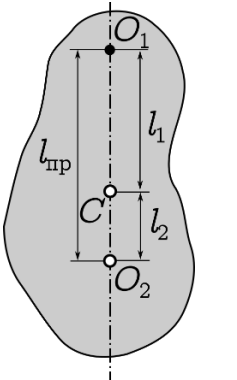
\includegraphics{Рис.1.png}
\end{figure}

where $l_{\text{r}}$ - reduced length.\\


\textbf{Huygens'theorem on the revolving pendulum}


Because of using Huygens'theorem we can write these formulas:
$$T_{1} = 2\pi\sqrt{\frac{I_{1}}{mgl_{1}}}, \quad T_{2} = 2\pi\sqrt{\frac{I_{2}}{mgl_{2}}} \quad (3)$$
$$I_{1} = I_{c} + ml_{1}^2, \quad I_{2} = I_{c} + ml_{2}^2 \quad (4)$$
where $I_{c}$ - the moment of inertia relative to point C.\\


\textbf{Measure g}

Let $L=O_{1}O_{2}=l_{1}+l_{2}$. If $T_{1}=T_{2}$, so $L=l_{\text{пр}}$. From (1) and (2) we can find g:
$$g_{0} = (2\pi)^2\frac{L}{T^2} \quad (5)$$

Exact match between $T_{1} = T_{2}$ is impossible to achieve. So let`s write formula for g, if periods have minor discrepancies: $T_{1}=T$ $T_{2}=T+\triangle T$. From (3) and (4) we can get:
$$g=(2\pi)^2\frac{l_{1}^2 - l_{2}^2}{T_{1}^2l_{1}-T_{2}^2l_{2}} \quad (6)$$
we can rewrite as
$$g=g_{0}\frac{\lambda - 1}{\lambda - \frac{T_{2}^2}{T_{1}^2}} \quad (7)$$
where $g_{0}=(2\pi)^2L/T^2$ and $\lambda = \frac{l_{1}}{l_{2}}$

Analyze the differences between (5) and (7). Let $\varepsilon =\frac{\triangle T}{T}\ll 1$ - relative deviation when measuring periods. So if $\lambda \neq 1$, using a little $\varepsilon$, we can get
$$g=g_{0}\frac{\lambda - 1}{\lambda - (1+\varepsilon)^2} \thickapprox g_{0}\frac{1}{1 - \frac{2\varepsilon}{\lambda - 1}} \thickapprox g_{0}(1+2\beta\varepsilon)$$
where
$$\beta \equiv \frac{1}{\lambda-1} = \frac{l_{2}}{l_{1}-l_{2}}$$

It can be seen that the amendment $\triangle g \thickapprox 2\beta\varepsilon g$ to formula (5) remains little if little $\varepsilon$, and the coefficient is little $\beta = \frac{l_{2}}{l_{1}-l_{2}}$. Therefore, in practice, it is desirable that $l_{1}/l_{2}>2,5$.\\

\textbf{Experimental setup}

\begin{figure}[h!]
    \centering
    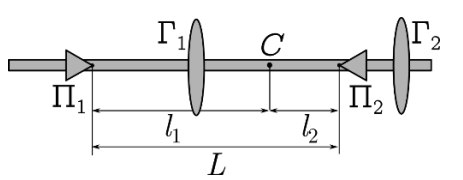
\includegraphics{2022-11-15.png}
\end{figure}

\textbf{\large Collecting data}\\

$m_{\text{г1}}=1495,8$ g, $m_{\text{г2}}=1484$ g, $m_{\text{п1}}=78,9$ g, $m_{\text{п2}}=79,6$ g, $m_{\text{ст}}=868,3$ g, $\sigma_{m}=0,5$ g\\

$L_{\text{ст}}=1000,6$ mm, $L=607,5$ mm, $\sigma_{L}=0,1$ mm\\

With the help of a $\bot$-shaped stand, it was possible to determine the location of the center of mass of the pendulum with loads, it turned out to be removed from the edge from the side of the load G2 at a distance of 372.7 mm.\\

Calculated using the formula \Large $\frac{\sum_{i}^n m_{i}x_{i}}{m_{i}}$ \normalsize Calculated using the formula of the center of mass was removed from the right edge at a distance of 373.2 mm. Thus, $l_{1}=432$ mm, а $l_{2}=175,5$ mm, $\sigma_{l}=1$ mm.\\

Pendulum oscillations when suspended for П2 (20 oscillations)\\

\begin{tabular}{c|c|c}
N & t,s & T,s\\
\hline
 1 & 31,22 & 1,561\\
 2 & 31,22 & 1,561\\
 3 & 31,14 & 1,557\\
 4 & 31,13 & 1,5565\\
\end{tabular}\\
\\

$T_{\text{ср}}$=1,558 s\\


Pendulum oscillations when suspended for П1 (20 oscillations)\\

\begin{tabular}{c|c|c}
N & t,s & T,s\\
\hline
 1 & 31,20 & 1,56\\
 2 & 31,20 & 1,56\\
 3 & 31,21 & 1,5605\\
 4 & 31,20 & 1,56\\
\end{tabular}\\

$T_{\text{ср}}$=1,56 s\\

Thus, \triangle T=0.002 \text{s},\; $\triangle T/T \thickapprox 0,001 $. The deviation is about 0.1\%. This indicates the correctness of determining the position of the goods. Now let's make the final measurement of the periods $T_{1}$ and $T_{2}$.\\

Pendulum oscillations when suspended for П2 (100 oscillations)\\

\begin{tabular}{c|c|c}
N & t,s & T,s\\
\hline
 1 & 155,52 & 1,5552\\
 2 & 155,5 & 1,555\\
 3 & 155,39 & 1,5539\\
\end{tabular}\\

Using the standard deviation formula, we obtain that $\sigma_{T2}^{\text{случ}}=0,0004$. Because $\sigma_{T}^{\text{сист}}=0,001$s, result $\sigma_{T2}\thickapprox 0,001$ s.\\

Pendulum oscillations when suspended for П1 (100 oscillations)\\

\begin{tabular}{c|c|c}
N & t,s & T,s\\
\hline
 1 & 155,99 & 1,5599\\
 2 & 155,97 & 1,5597\\
 3 & 156,02 & 1,5602\\
\end{tabular}\\

$\sigma_{T1}^{\text{случ}}=0,00015$ s, $\sigma_{T1}\thickapprox 0,001$ s.\\

Thus, $T_{1}=T=1,560\pm 0,001$ s, $T_{2}=T+\triangle T= 1,554\pm 0,001$ s.\\

\textbf{\large \text{Вычисление ускорения свободного падения}}\\

Using formula (6) to determine g, we get that g =9.8187 m/s2. To calculate the error g , we use the formula:
$$\sigma_{g} =g\sqrt{(\frac{\sigma_{L}}{L})^2+4(\frac{\sigma_{T}}{T})^2+8(\beta\frac{\sigma_{T}}{T})^2+8(\beta\frac{\triangle T}{T}\frac{\sigma_{L}}{\triangle l})^2} $$\\
where $\triangle l=l_{1}-l_{2}$ and $\triangle T=T_{1}-T_{2}$. So we get $\sigma_{g} = 0,0176$ m/s2 and \large $\frac{\sigma_{g}}{g}  \thickapprox 0,2\%.$\\

g\thickapprox9,82\pm 0,02\; \text{m/s2} \\

It is possible to calculate the error in calculations using the formula (6), using standard rules. Result $\sigma_{g} = 0,0314$ m/s2, тогда $g\thickapprox9,82\pm0,03$ m/s2 and $\frac{\sigma_{g}}{g}\thickapprox0,3\%$.

\textbf{\large Conclusion}

We have measured with high accuracy the magnitude of the acceleration of free fall.

\end{document}
